% !TeX spellcheck = en_US
\section{Problem 6}

This problem depends on Problem 5, as it uses its technique to train a neural network.
The only thing changing here is the \verb|generate_AR_data()| function, that now creates a time series that is described using the following equation:
\[
X_t = U_t + a_1 U_{t-1} + a_2 U_{t-2} + a_3 U_{t-3} + a_4 U_{t-4} + a_5 U_{t-5} + a_6 U_{t-6}
\]
with $a_1 = a_2 = 5$ and $a_3 = a_4 = a_5 = a_6 = -0.5$.

\begin{minipage}{0.48\linewidth}
	\centering
	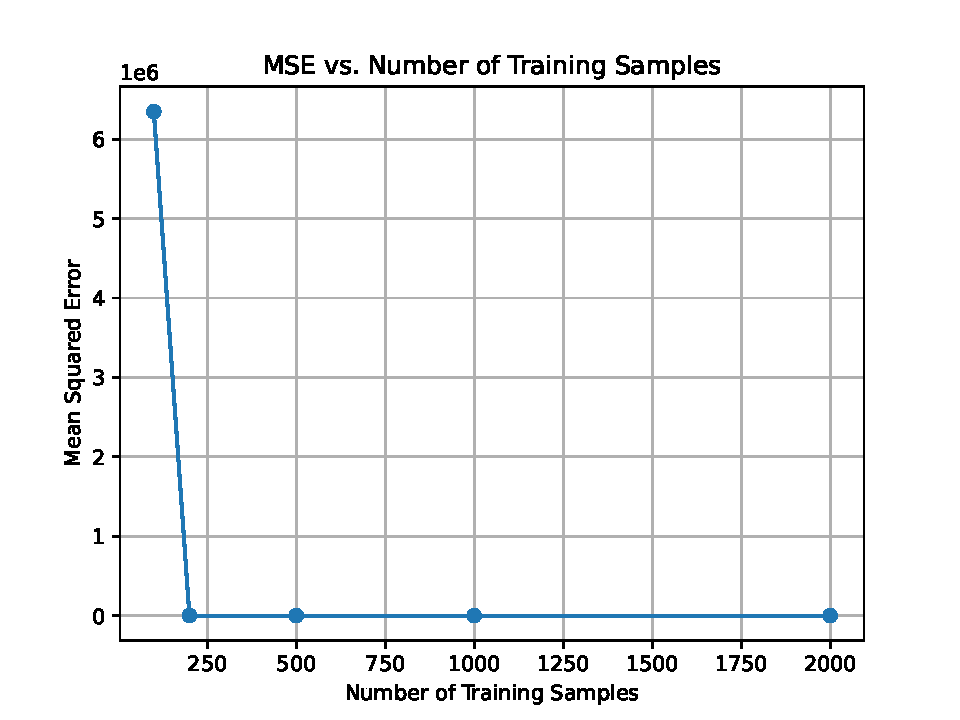
\includegraphics[width=\linewidth]{../Problem 6/prob6_mse_vs_total_epoch.pdf}
	\captionof{figure}{Averaged cost square error function over number of training samples}
	\label{fig:prob6_mse_total_epoch}
\end{minipage} \hfill
\begin{minipage}{0.48\linewidth}
	\centering
	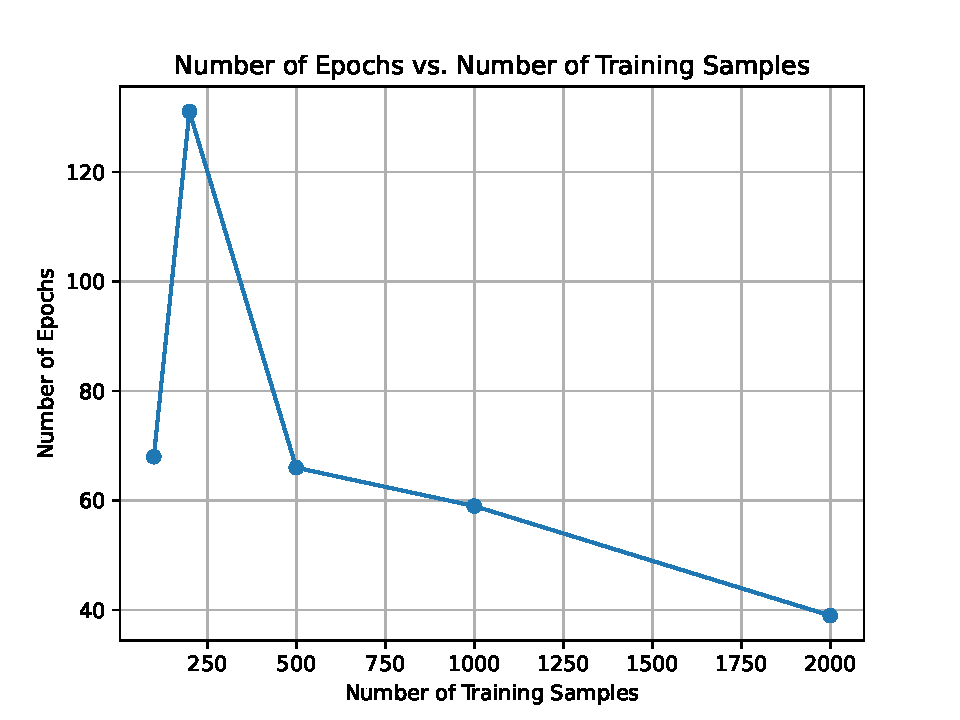
\includegraphics[width=\linewidth]{../Problem 6/prob6_epoch_vs_training_samples.pdf}
	\captionof{figure}{Number of epochs required for the NN to converge}
	\label{fig:prob6_epoch_train_samples}
\end{minipage}
